\pagestyle{fancy}

\begin{abstract}
The HIVE AURC Avionics (Data Analytics and Verification) capstone project was formed as part of RMIT HIVE's endeavours to compete in the 2024 Australian Universities Rocket Competition. Participants in this project acted as a part of the Aurora V avionics team, with the focus on developing systems for data analytics on the rocket, including the firmware implementation for real time processing and communications of data during flight, as well as avionics systems testing for verification.
\end{abstract}

\section{Introduction}


\subsection{Background}
The Australian Universities Rocket Competition (AURC) is one of Australia’s competitions for university student teams to design, build, and launch high-powered model rockets. The AURC is organised to encourage students from across Australia to develop technical and project management skills in aerospace engineering. Participating teams are required to launch rockets to specific altitudes, either 10,000 feet or 30,000 feet while integrating payloads and avionics systems that can capture and transmit real-time flight data. 

The competition is a significant platform for enabling innovation in aerospace technology, particularly focusing on rocketry, avionics, and data analytics. Teams are evaluated not only on the rocket’s performance but also on their design, safety considerations, and the accuracy of data acquisition during flight. 

A key focus area for the Aurora rockets has been the development of a reliable avionics system capable of handling the demands of high-speed, high-altitude flights. The Aurora V rocket, designed for the 2024 AURC, was expected to reach an apogee of 10,000 feet and relied on a custom avionics system for monitoring and controlling its flight. This competition not only pushes the technical boundaries of rocketry but also provides opportunities for students to engage in real-world engineering challenges. 

\begin{figure}[h]
    \begin{center}
        
\includegraphics[width=0.95\textwidth]{./img/subsystems_avionics.png}
    \end{center}
    \caption{Aurora Project subsystems}\label{fig:subsystems_avionics}
\end{figure}

The Aurora V team consisted of 30 students from various disciplines, including aerospace engineering, mechatronics, electronics, computer science and biomedical. The team is structured into several sub teams, each responsible for different aspects of the rocket’s design and performance. These sub teams include Avionics, Aerostructures, Ground Communications, Payload, Recovery and Aerobrakes -- as pictured in Figure~\ref{fig:subsystems_avionics}. The Data Analytics and Verification team, as a subset of the Avionics team, worked closely with these groups to ensure seamless integration of the custom hardware and firmware developed for flight monitoring and data analysis. This multidisciplinary collaboration enabled the Aurora V team to address complex engineering challenges from different engineering perspectives and deliver a rocket system that meets the requirements of the AURC competition. 

The Data Analytics and Verification team was responsible for not only gathering sensor data but also ensuring its accuracy through validation and real-time analysis. The team worked closely with the Avionics, Ground Communications, and Redundant Systems team, which was tasked with designing and building the custom hardware required for the avionics system. Meanwhile, the Data Analytics and Verification team focused on designing and implementing the custom firmware that enables sensor fusion, state estimation, telemetry, and communications between subsystems. 

This division of scope allowed for the ease of integration between the hardware and firmware, easing development across the board for the avionics team. Given the complexities involved in high-powered rocket flights, where the environment is constantly changing, this team was key in ensuring that flight data is accurate and can be used for both in-flight decisions and post-flight analysis. The team’s efforts are geared toward creating a more reliable and fault-tolerant avionics system that enhances the overall performance of the Aurora V rocket in the AURC. 

The final competition launch, initially planned to take place in Western Australia, was unfortunately cancelled due to logistical challenges, particularly the inability to secure rocket motors in time for the event. As a result, the AURC shifted to an online format, where teams would present their designs, systems, and findings rather than conducting a physical launch. In this modified competition format, the objective of the Data Analytics and Verification team has expanded to include providing comprehensive systems documentation and findings for future RMIT teams. 

These future teams will build on the groundwork laid by the current Aurora V team and aim to successfully compete in the next AURC and beyond by taking advantage of the avionics systems and data validation processes and findings developed during this project. 

\subsection{Problem Statement}
The primary challenge for the Data Analytics and Verification team was to design, implement, and validate data analytics and real-time verification processes for the Avionics system of the Aurora V rocket, which was expected to fly in the 2024 Australian Universities Rocket Competition (AURC). The avionics system, developed by the Avionics, Ground Communications, and Redundant Systems team, presents significant constraints, including limited processing power, memory, and communication bandwidth.

\begin{figure}[h]
    \begin{center}
        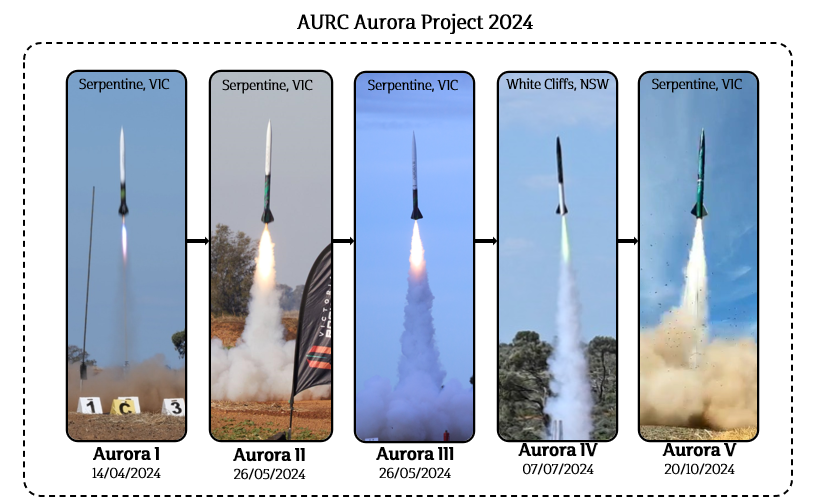
\includegraphics[width=0.95\textwidth]{./img/aurora.png}
    \end{center}
    \caption{Aurora project timeline}\label{fig:aurora}
\end{figure}

These limitations needed to be considered while ensuring the collection, logging, and real-time analysis of sensor data in-flight. Additionally, the Data Analytics and Verification team needed to ensure the accuracy of telemetry and state estimation to support critical flight functions such as the aerobrake control system and recovery mechanisms. The challenge extended to testing these systems across multiple rocket iterations (Aurora I to V as pictured in Figure~\ref{fig:aurora}), ensuring that improvements were made with each launch.

\subsection{Project Deliverables}
For the major portion of this capstone, the objectives and deliverables were maintained. The following objectives and deliverables aim to delineate between objectives of the AURC and this capstone project team.

\begin{enumerate}
    \item \textbf{Data Capture and Logging Implementation}: Develop firmware to define sampling rates and intervals for sensor data capture and establish reliable logging formats for storage and later analysis.
    \item \textbf{Real-Time Data Processing}: Design algorithms for sensor fusion, incorporating multiple sensor inputs to produce accurate state estimation. Implement filtering techniques (e.g., Kalman filters) to reduce noise which is critical for the aerobrake control system.
    \item \textbf{Post-Processing and Analysis}: Conduct post-flight statistical analysis to evaluate the performance of avionics systems. Detect deviations from expected behaviour, comparing raw sensor data with processed, fused data. Compare results against the Blue Raven flight computer to ensure accuracy.
    \item \textbf{Data Visualisation}: Develop tools to visualise data, generating graphs and charts that allow for clear interpretation of results. This also includes the potential for creating flight simulations based on collected data.
    \item \textbf{Data Validation}: Implement verification processes to assess the validity and integrity of captured data. This includes identifying and addressing data errors, hardware malfunctions, and inconsistencies.
\end{enumerate}

\subsection{Project Scope}
The Data Analytics and Verification team operates within the Avionics subsystem and focuses on the following key activities:

\begin{enumerate}
    \item \textbf{Software Development}: Design and develop firmware responsible for data collection, logging, and real-time processing. Post-processing involves visualising and analysing the collected data to detect anomalies and verify system performance.
    \item \textbf{Algorithm Development}: Research and implement sensor fusion, filtering (using techniques like the Kalman filter), and state estimation algorithms to ensure accurate in-flight data.
    \item \textbf{Testing and Validation}: Perform ground-based and in-flight testing (Aurora I to V) to validate the reliability and performance of the data analytics system. Each launch provides opportunities to refine the system based on feedback.
    \item \textbf{Iterative System Refinement}: Continuously refine the firmware and analysis algorithms based on data collected from each rocket iteration. This culminates in a competition-ready avionics system for Aurora V. Although the final Aurora V launch will not be part of the official competition, the findings and outcomes will contribute valuable insights for future students and teams, ensuring continuity and further development of the system for subsequent launches.
\end{enumerate}


\section{Literature Review}
\subsection{Data Analytics in Avionics}
Data analytics in rocketry, particularly within avionics systems, has become a significant component as rockets evolve with increasingly complex sensor suites and intricate flight dynamics. Data analytics refers to the systematic collection, processing, and interpretation of data generated by a rocket's avionics system throughout pre-flight, in-flight, and post-flight operations. The ability to analyse and interpret this data in real-time is key for monitoring critical parameters such as altitude, velocity, acceleration, and orientation, which are used to control flight dynamics, initiate recovery systems, and make real-time adjustments. Post-flight data analysis further contributes to system optimisation by identifying deviations and improving future launches through data analysis. 

\subsection{State Estimation Techniques}
\subsection{Real-Time Operating Systems (RTOS) in High Powered Rockets}
\subsection{Testing and Verification in Rocketry}

\subsubsection{Barometer and Vacuum Chamber Testing}
In rocketry, precise altitude measurement is essential for triggering key events, primarily the deployment of the recovery parachute. Barometric sensors, which measure air pressure to estimate altitude, are widely used for this purpose. To validate their performance under controlled conditions, vacuum chamber testing is a common method. This testing simulates the pressure changes a rocket would experience during ascent, allowing engineers to verify that the barometer accurately responds to varying altitudes and pressure changes. 

One study used a vacuum chamber to simulate altitudes ranging from 75 to 2100 meters, testing altimeters for their accuracy across these ranges \cite{NAR-58}. By correlating the chamber's pressure changes with expected altitude measurements, the study was able to validate both passive sensor monitoring and active sensor emulation methods. These tests are crucial to ensure that the barometers function reliably during flight and respond appropriately to dynamic environmental conditions, such as pressure fluctuations caused by wind or rapid altitude changes.

In rocketry, precise altitude measurement is essential for triggering key events, primarily the deployment of the recovery parachute. Barometric sensors, which measure air pressure to estimate altitude, are widely used for this purpose. To validate their performance under controlled conditions, vacuum chamber testing is a common method. This testing simulates the pressure changes a rocket would experience during ascent, allowing engineers to verify that the barometer accurately responds to varying altitudes and pressure changes. 

One study used a vacuum chamber to simulate altitudes ranging from 75 to 2100 meters, testing altimeters for their accuracy across these ranges. By correlating the chamber's pressure changes with expected altitude measurements, the study was able to validate both passive sensor monitoring and active sensor emulation methods. These tests are crucial to ensure that the barometers function reliably during flight and respond appropriately to dynamic environmental conditions, such as pressure fluctuations caused by wind or rapid altitude changes.

\subsubsection{Accelerometer and Gyroscope Testing}
In addition to the barometer, accelerometers and gyroscopes are key sensors used in rocketry to measure acceleration and angular velocity, respectively. These sensors provide important data for calculating the rocket's velocity, orientation, and trajectory. Ground testing of accelerometers typically involves placing the sensor in a controlled motion environment where its output can be compared against known values. For instance, flight motion simulators can recreate the conditions experienced during rocket flight, including G-forces and rapid directional changes. These setups allow engineers to calibrate the sensors, ensuring that their outputs remain accurate under high stress conditions.  

Inertial Measurement Units (IMUs), which combine accelerometers and gyroscopes, are also extensively tested in rocketry. These tests often involve multi-axis rate tables, which can simulate complex flight dynamics in multiple directions. Testing these systems helps in detecting sensor biases, misalignments, and nonlinearities.  The calibration process ensures that IMUs can accurately capture data that will be used for flight control and telemetry.  

\subsubsection{General Testing in Rocketry}
Beyond sensor-specific tests, rocket avionics systems undergo extensive testing to validate their performance under the high-stress environments experienced during flight. These systems must reliably operate under extreme conditions, such as high G-forces, vibrations, and rapid velocity changes. Ground-based tests are critical for identifying potential system failures before launch. One common approach is telemetry reliability testing, which ensures that real-time data transmission remains uninterrupted, even when the rocket reaches high speeds and altitudes. This process often uses radio frequencies, such as Xbee modules, to transmit data between the rocket and the ground station \cite{rocket_telemetry}.

One technique used is Hardware-in-the-Loop (HIL) simulations, to validate avionics systems in controlled environments. HIL simulations integrate the rocket's actual hardware, such as flight computers or controllers, with simulated inputs and outputs to replicate real flight conditions without exposing the rocket to the physical stresses of an actual launch. This method allows engineers to subject the system to various scenarios, including fault injection tests where simulated sensor failures or unexpected conditions are introduced to test the system’s resilience \cite{HIL_rocket, HIL}. 

For example, by using HIL simulation, engineers can test the rocket's response to potential sensor failures during flight. These simulations help in understanding how the avionics system would behave in nominal and off-nominal situations, such as when a sensor provides erroneous data or fails completely \cite{HIL_rocket}. 

In rocketry, this is particularly useful in identifying vulnerabilities that could lead to major failures. Additionally, precise calibration of the telemetry and control systems through HIL simulation ensures repeatability and consistency in the rocket's performance.

\section{Implementation and Design Justification}
\subsection{Aurora I and II}
Due to delays in hardware availability from vendors, the Aurora I avionics system was constructed using a minimalistic or "bare bones" design, incorporating only the most essential components that were readily available. Despite the limitations, the Aurora I system still enabled the team to test critical functionalities, such as sensor data capture and storage on flash memory. Although it did not meet the original Aurora I design goals, the system provided a valuable opportunity for the team to develop fundamental capabilities, which were pivotal in guiding the design of future systems, particularly for Aurora III. 

The avionics design for Aurora I primarily focused on creating a foundational framework for gathering and storing flight data. It served as a proof of concept for using custom electronics with an Arduino-based system for data logging and sensor integration. Despite the absence of more advanced features such as real time telemetry, the system gathered preliminary flight data that informed later iterations of the rocket's avionics system and provided real world data to formulate state estimations techniques.  

\subsubsection{Avionics Design Overview}
The Aurora I avionics system consisted of two main components:

\begin{itemize}
    \item \textbf{Commercial Off-The-Shelf (COTS) Blue Raven Flight Computers}: These were responsible for activating the drogue and main parachutes for recovery. Additionally, they recorded flight data, which was used for post-flight analysis.
    \item \textbf{Custom Avionics Board}: Built on a perfboard, this board housed an Arduino Nano microcontroller and several sensors, including an accelerometer, barometer, gyroscope, and magnetometer. These sensors provided data on the rocket's altitude, orientation, and velocity, all of which were essential for assessing flight dynamics. The Arduino Nano controlled data acquisition and storage, while a SerialFlash module was used to store sensor data onboard for later retrieval.
\end{itemize}

Key objectives of the Aurora I design were to:

\begin{itemize}
    \item Gain practical experience with the COTS Blue Raven flight computers.
    \item Test various battery configurations, sensor data collection, and flash memory storage in flight conditions.
    \item Capture flight data for post-flight analysis to improve avionics design for subsequent iterations.
\end{itemize}

\subsubsection{Firmware Architecture}
The high-level flow chart provided under Appendix~\ref{apdx:flowchart_a1} depicts how the Aurora I avionics system captures and transmits data. The primary goal was to facilitate post-flight analysis and verification, aligning with the data collection intervals of the Blue Raven system (500 Hz high resolution and 50 Hz low resolution). Due to timing constraints as a result of lesser performant hardware for Aurora I, the high-resolution interval was elected to operate at 250 Hz to ensure all processes have adequate time to complete. Data logging was initiated by a launch event detected when vertical acceleration exceeds a pre-defined threshold (5g at present). During flight, raw sensor data was stored onboard in flash memory. 

\paragraph{High Resolution Data Capture}

The high resolution interval (250 Hz) focuses on data from an Inertial Measurement Unit (IMU), comprising accelerometer, gyroscope, and magnetometer sensors. This high sampling rate is used to accurately capture subtle changes in aircraft motion and orientation. Raw data from sensor registers is combined with headers into data frames, stored in a buffer, and then written to flash memory. 

\paragraph{Low Resolution Data Capture and Transmission}

The low resolution interval (50 Hz) reads data from a barometer (pressure and temperature sensor) to determine altitude. Similar to the high resolution process, raw data is framed and temporarily stored in a buffer before writing to flash.  

\paragraph{Design Considerations and Implementation}

Alternative design approaches were considered, including a separate logging interval. However, the chosen design simplifies the system by consolidating flash writing and LoRa transmission into the low resolution interval. This streamlines data handling tasks while still meeting the core requirements. Although LoRa communications was included in the initial Aurora I software design, the hardware to support this was unavailable at the time due to delays in hardware delivery. As a result, testing for LoRa communications was organised to be implemented in Aurora II. 

\paragraph{Development Testing and Optimisation}

During initial tests, it became apparent that there were significant delays in accessing sensor data, especially when handling the sensors at high frequencies. These delays are depicted in timing tests (Figure~\ref{fig:sensor_timing-A1}), where it was found that accessing data from the sensors was too slow to meet the system’s real-time data capture requirements. The primary cause of this issue was traced back to the overhead created by the sensor libraries, many of which included non-essential features that added unnecessary processing time, in addition to the sensor's communication interface -- all devices with the exception of flash storage communicated on an I2C bus which typically has greater overhead than other interfaces with the benefit being its connectivity. 

\begin{figure}[h]
    \begin{center}
        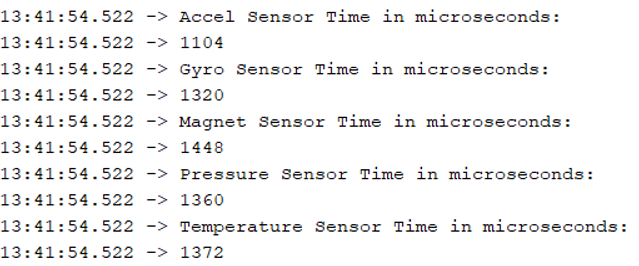
\includegraphics[width=0.85\textwidth]{./img/sensor_timing-A1.png}
    \end{center}
    \caption{Measurements of sensor read time for Aurora I}\label{fig:sensor_timing-A1}
\end{figure}

To address this, the team conducted a series of optimisation tests. These tests involved stripping back the libraries to include only the core functionalities necessary for flight operations. The library optimisations resulted in significantly reduced sensor access times, however the total processing time for high resolution sampling very barely fell within the requirements for a $\qty{500}{\hertz}$ interval and it was as such decided to leave the sampling rate at $\qty{250}{\hertz}$ as a precaution.

\subsubsection{Data Storage and Handling}

\subsection{Aurora III to V}
\subsubsection{Avionics Design Overview}
The Aurora III avionics system was designed to manage power, acquire flight and payload data, facilitate internal vehicle communication, and enable vehicle-to-ground communication. However, when compared to Aurora I and Aurora II, it also plays an additional role in supporting the Aerobrakes and Recovery subsystems by providing essential flight data which includes altitude and velocity. Ground communication through LoRa protocol is also included within the systems, supporting live state estimates during flight. The hardware is equipped with a complete sensor suite comprising of an accelerometer, gyroscope and barometer, on board flash, and both a GPS and LoRa communications module optimised with by a Real-Time Operating System or RTOS prioritising the critical task.   

The system uses an STM32F439 microcontroller as its core processing unit. This microcontroller was chosen by the broader team for its familiarity, sufficient clock speed, ample I/O pins, and built-in SPI/I2C and CAN bus functionality. The addition of LoRa communication enables real-time data transmission to the ground station, enhancing monitoring and analysis capabilities. The system also incorporates the ability to receive and send data to the payload and aerobrakes subsystems via the CAN 2.0A protocol, facilitating integrated control and decision-making during flight. 

% TODO: avionics board figure

Aurora V improves from this design, comprising of two SRAD (Student-Research and Developed) flight computers, while maintaining inter-subsystems communications and telemetry functionally. These two flight computers are connected via a communications bus that facilitates the transfer of system state data. During flight, one computer serves as the primary controller. However, in the event of a partial system failure, control is automatically shifted to the redundant computer transferring primary controls. 

\begin{figure}[h]
    \begin{center}
        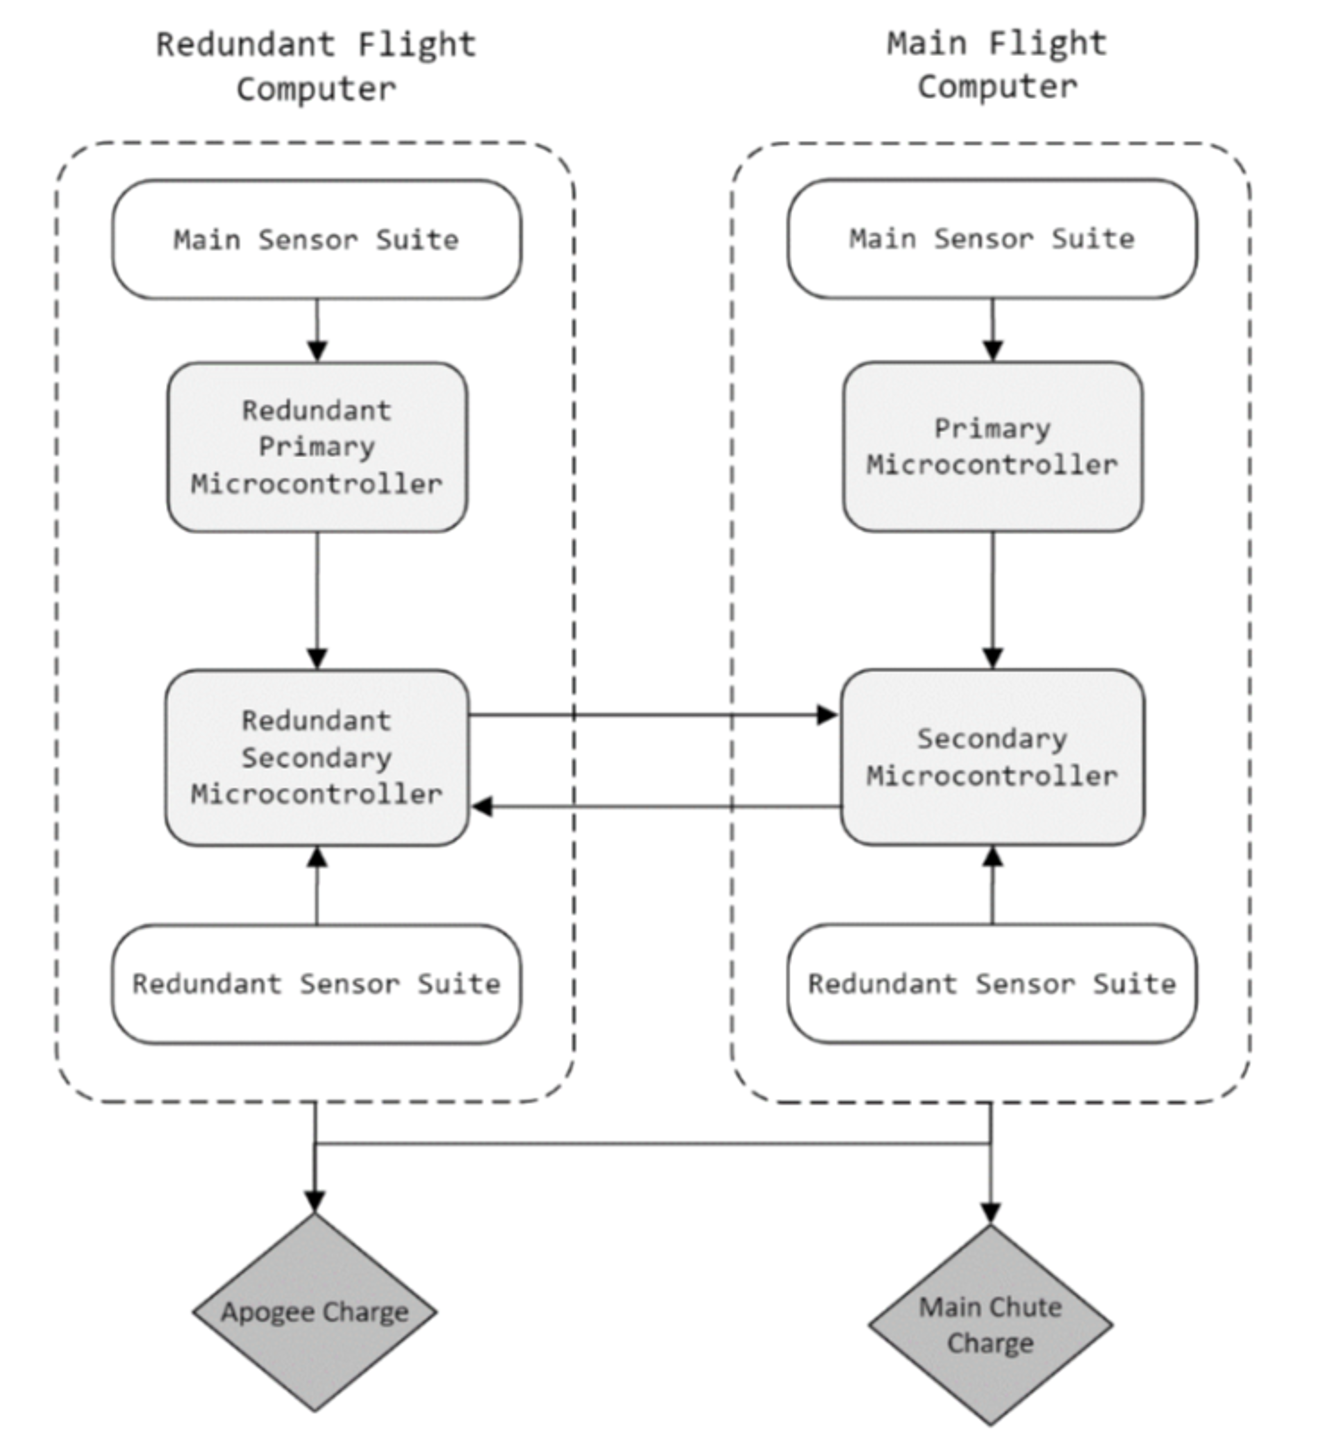
\includegraphics[width=0.75\textwidth]{./img/redundancy.png}
    \end{center}
    \caption{Aurora V Avionics system, designed by the Ground Communications and Redundant Systems team \cite{avionics}}\label{fig:redundancy}
\end{figure}

% TODO: rewrite
Each flight computer is equipped with its own sensor suite, allowing both to independently determine the vehicle’s state. To initiate drogue parachute deployment at apogee, both microcontrollers participate in a voting process. The secondary microcontroller will activate recovery once at least two apogee detection votes are confirmed, ensuring a fail-safe mechanism for recovery deployment. A block diagram illustrating the high-level design of the Aurora V avionics redundancy system is shown in Figure~\ref{fig:redundancy}.

\subsubsection{Firmware Architecture Design and implementation}

With the development of a new avionics board for the flight of Aurora III, significant improvements to the firmware systems were identified as a necessity. While the previous flight computer simply logged data from sensors in a looping process, the eventual goal of the team's custom avionics was to support SRAD recovery deployment, inter-rocket communications with other subsystems, ground station telemetry, real time data processing, as well as data logging.

With these requirements in mind, the team chose to move to a firmware implementation with in-house developed hardware drivers, supported by a backbone of FreeRTOS to provide a real-time scheduling system for these tasks to operate within. The benefit of such a design is the team has near complete control over the code running on system hardware, allowing for better insight into its operation when it comes to error diagnostics. 

Additionally, with the significantly increased list of requirements compared to previous rocket iterations, the use of an RTOS simplifies firmware development by allowing the isolation of tasks with real-time synchronisation features to support inter-process communication.

With the exception of core startup code and the RTOS scheduler, all libraries used within the firmware were developed by the team from the ground up, including the custom avionics library with included packages for quaternion calculations, Kalman Filter implementation, and memory buffer management.

% Lol stupid dumb mf hack
\subsubsection*{\hspace{4.2em}RTOS architecture}

\begin{figure}[h]
  \centering
  \begin{tikzpicture}[
      node distance=0mm and 3mm,
      task/.style={rectangle, minimum height=6mm, rounded corners, draw=black!75, radius=5pt, anchor=west},
      tier/.style={rectangle, draw=black, minimum width=10cm, minimum height=1cm, anchor=west},
    ]
    \node (health) [task, xshift=2mm] {Health Monitor};
    \node (tierCRITICAL) [tier, label=left:{\color{red}CRITICAL}] {};

    \node (flash) [task, below=of health.south west, anchor=north west, yshift=-0.4cm] {Flash Write};
    \node (CANTx) [task, right=of flash] {CAN Tx};
    \node (tier-1) [tier, below=of tierCRITICAL, label=left:-1] {};

    \node (HDataAcq) [task, below=of flash.south west, anchor=north west, yshift=-0.4cm] {High Res Data Acquisition};
    \node (tier-2) [tier, below=of tier-1, label=left:-2] {};

    \node (LDataAcq) [task, below=of HDataAcq.south west, anchor=north west, yshift=-0.4cm] {Low Res Data Acquisition};
    \node (tier-3) [tier, below=of tier-2, label=left:-3] {};

    \node (state) [task, below=of LDataAcq.south west, anchor=north west, yshift=-0.4cm] {State Management};
    \node (tier-4) [tier, below=of tier-3, label=left:-4] {};

    \node (LoRa) [task, below=of state.south west, anchor=north west, yshift=-0.4cm] {LoRa Tx};
    \node (CANRx) [task, right=of LoRa] {CAN Rx};
    \node (tier-5) [tier, below=of tier-4, label=left:-5] {};

    \node (flashEN) [task, below=of LoRa.south west, anchor=north west, yshift=-0.4cm] {Flash enable};
    \node (idle) [tier, below=of tier-5, label=left:{\color{blue}Idle}] {};

    \draw[arrows = {Latex-Latex}] ([xshift=4mm]tierCRITICAL.north east)--node[label, right]{Priority}([xshift=4mm]idle.south east);
  \end{tikzpicture}
  \caption{Avionics RTOS task hierarchy}\label{fig:priority}
\end{figure}

Figure~\ref{fig:priority} outlines the task architecture that was designed prior to beginning work on the system, with tasks more critical to operation placed towards the top. These tasks can be broken down into subcategories as such: 
\begin{itemize}
    \item Data acquisition and processing
    \item Data storage
    \item Communications
\end{itemize}

Not included in this category list is the health monitor which is yet to be fully realised within the system. The sections following will break down each of these categories and their role within the avionics system.

\paragraph{Data acquisition and processing} these tasks constitute the sampling of sensors as well as critical calculations of flight data in real time. 

This data is used post-flight for analysis, however more importantly it is used in the determination of critical phases of flight and actuation of systems internal to the rocket.\\

\begin{lstlisting}[escapeinside=``, caption={High resolution quaternion calculations}, captionpos=b, label={lst:highres}]
// Integrate attitude quaternion from rotations
Quaternion qDot;
Quaternion_init(&qDot);
qDot.fromEuler(
    &qDot,
    (float)(dt * gyro->gyroData[ROLL_INDEX]),
    (float)(dt * gyro->gyroData[PITCH_INDEX]),
    (float)(dt * gyro->gyroData[YAW_INDEX])
);
*qRot = Quaternion_mul(qRot, &qDot);
qRot->normalise(qRot); // New attitude quaternion

// Apply rotation to z-axis unit vector
qRot->fRotateVector3D(qRot, vLaunch, vAttitude);

// Calculate cosine
*cosine = vLaunch[0] * vAttitude[0] 
        + vLaunch[1] * vAttitude[1] 
        + vLaunch[2] * vAttitude[2];

// Calculate tilt angle
*tilt   = acos(*cosine) * 180 / M_PI;
\end{lstlisting}

The high resolution data is sampled at a rate of $\qty{500}{\hertz}$ -- equal to the high rate frequency of the Blue Raven -- within a periodic task. Per interval, each of the two on-board accelerometers as well as the gyroscope are polled for the latest data updated within their registers. The drivers for these sensors collect raw data and process it, storing both readings in memory for internal use.

% TODO: provide data on execution time 
Following the sampling of these sensors, the gyroscopic rates are further processed into quaternions, using the code shown in Listing~\ref{lst:highres} and the rocket body tilt and tilt angle cosine are calculated. 

These parameters are used in apogee detection and also by the aerobrakes to force retract the blades upon a tilt angle greater than $\qty{30}{\degree}$.\\

\begin{lstlisting}[escapeinside=``, caption={Low resolution state calculations}, captionpos=b, label={lst:lowres}]
// Calculate altitude
*altitude = 44330 * (1.0 - pow(baro->press / baro->groundPress, 0.1903));
`\Suppressnumber`
...
`\Reactivatenumber`
// Calculate state
z.pData[0] = *altitude;
z.pData[1] = (*cosine * 9.81 * accel->accelData[ZINDEX] - 9.81);

// Update filter
kf.update(&kf, &z);

// Retrieve velocity
*velocity = kf.x.pData[1];
\end{lstlisting}

The low resolution task samples only the barometer at a rate of $\qty{50}{\hertz}$, again identical to that on the Blue Raven. The pressure value is sampled, again with the driver maintaining both raw and processed values in memory, and the altitude is calculated. 

A Kalman Filter is run (Listing~\ref{lst:lowres}) to estimate the rocket's vertical velocity with altitude and acceleration as input measurements, using the previously calculated tilt angle cosine to rotate the acceleration from the rocket's body frame of reference to the earth's frame of reference.

Following the low resolution data acquisition, at a lower priority, a state update task is scheduled to manage the current system state using parameters calculated previously. An internal state machine is iterated to check the current phase of flight, and using the latest data determines if a state transition has occurred. 

\begin{figure}[h]
    \begin{center}
        \begin{minipage}{0.48\textwidth}
            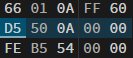
\includegraphics[width=\linewidth]{./img/coast_frame.png}
        \end{minipage}\hspace{1em}%
        \begin{minipage}{0.48\textwidth}
            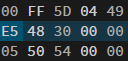
\includegraphics[width=0.92\linewidth]{./img/apogee_frame.png}
        \end{minipage}
    \end{center}
    \caption{(Left) Binary representation of coast event with header 0xD5 and (Right) Binary representation of apogee event with header 0xE5}\label{fig:state_dataframes}
\end{figure}

On entering a new state, the task sends off any critical communications and logs an event with a timestamp (pictured Figure~\ref{fig:state_dataframes} for post-processing analysis.

Each data acquisition task additionally appends raw data samples from the sensors to a dataframe with an identifier, allowing the data to later be flashed by the storage handler tasks.

\paragraph{Data storage}
Data storage is handled by two tasks, where one runs at idle priority and enables the second task -- responsible for executing the flashing of data -- when it has available time on the CPU. The flash write task operates at top priority to prevent pre-emption from other tasks, where tasks of higher priority take over time on the CPU as they wake. 

This design allows the firmware to write data to flash whenever there is nothing else being computed, whilst still ensuring each individual write operation occurs without disruption. The data written to flash is stored within a circular buffer designed specifically for memory writes. This buffer tracks the state of three pointers: a head and tail pointer mark the start and end of a single $\qty{256}{\byte}$ page within the buffer, with an additional pointer that references the current cell being written.

% TODO add flowchart/diagram

When new data is added to the buffer, the cell pointer increments and the length count of the buffer is increased. If the length is greater than a single page width, the buffer is marked as ready for write, allowing the current page to be flushed out of the buffer and written to flash. Even if the page remains unflushed, the cell pointer continues to increment as new data is added to the buffer. If a buffer overrun occurs, the cell pointer wraps to the beginning, and if it continues eventually past the page head it will slide the entire page window forwards with each append.

Data is flushed from the buffer a single page at a time by the flash write task. When enabled by the idle task, the page will be written into an output buffer which is then iterated over and sent to the flash chip via its respective driver.

\paragraph{Communications}
The communications tasks handle the passing of messages across CAN, LoRa, and USART. Each message type has associated transmit and receive tasks with respective message buffers. These tasks simply wait for a message to arrive in the buffer and handle them appropriately. The transmit tasks will retrieve a message from the buffer as it arrives and send it out on the relevant interface, while receive tasks pull messages from the buffer and parse them.

On a fixed $\qty{500}{\milli\second}$ interval, a LoRa sample task will trigger to sample current avionics data to send to the ground station -- including current flight state, state of external connection to the Payload system, and raw flight data. This is then packaged as a message and delivered to the transmit task.

The CAN tasks primarily handle the communication between Avionics and Aerobrakes, as well as Payload. The Payload sends data to avionics to transmit over LoRa on request over CAN, which occurs at a similar fixed interval of $\qty{500}{\milli\second}$, and the data is added as another message that is appended to the LoRa transmit buffer. Aerobrakes messages are sent at key stages of flight, with continuous transmissions of altitude on every state update interval following the start of the coast phase, as well as a retract message sent when tilt exceeds $\qty{30}{\degree}$.

The CAN transmission task is implemented as high priority to ensure maximum responsiveness to the Aerobrakes such that the key deployment event is not missed or delayed.

\subsubsection{Data Processing}
The calculations performed by the avionics system during flight provide critical information on system state parameters, giving information on the rocket's flight dynamics. These calculations are critical for analysis on the performance of flights, as well as providing key data to other subsystems.

In order to maintain knowledge of the rocket's orientation relative to the earth's frame of reference, gyroscopic rates are integrated into attitude quaternions which are applied to the initial launch vector.

The instantaneous angular rate measurements output by the gyroscopic sensors can be considered as time derivatives of the Euler angle representation of the rocket's attitude. With these rates, rotation quaternions can be constructed through a method akin to numerical integration:\\[0.5em]
{
\setlength{\belowdisplayskip}{5pt}%
\setlength{\abovedisplayskip}{-15pt}%
\begin{align*}
  \intertext{First the angular rates in $\unit{\degree}/\unit{\second}$ are converted to Euler angles (radians):}\\
  \begin{bmatrix}
    \phi\\\theta\\\psi
    \end{bmatrix} &= \frac{\pi}{180}\cdot\begin{bmatrix}
                                        \omega_x\\\omega_y\\\omega_z
                                        \end{bmatrix}\\
    \intertext{A unit quaternion is then initialised through the half Euler angles (per equation 66 ~\cite{Diebel2006})}\\
    \dot q &= 
    \begin{bmatrix}
      c_{\phi/2}c_{\theta/2}c_{\psi/2}-s_{\phi/2}c_{\theta/2}s_{\psi/2}\\
      c_{\phi/2}c_{\theta/2}c_{\psi/2}+s_{\phi/2}s_{\theta/2}s_{\psi/2}\\
      c_{\phi/2}s_{\theta/2}s_{\psi/2}-s_{\phi/2}c_{\theta/2}s_{\psi/2}\\
      c_{\phi/2}c_{\theta/2}s_{\psi/2}+c_{\phi/2}c_{\theta/2}s_{\psi/2}\\
    \end{bmatrix}\\[0.5ex]
    \intertext{Where $c_x=\cos{x}$, $s_x=\sin{x}$. Then from equation 102~\cite{Diebel2006}:}\\
    q_{k} &= q_{k-1}\cdot\dot q\\
          &= \begin{bmatrix}
            (q_{{k-1}_0}  \dot q_0) + (-q_{{k-1}_1}  \dot q_1) + (-q_{{k-1}_2}  \dot q_2) + (-q_{{k-1}_3}  \dot q_3)\\
            (q_{{k-1}_0}  \dot q_1) + (q_{{k-1}_1}  \dot q_0) + (q_{{k-1}_2}  \dot q_3) + (-q_{{k-1}_3}  \dot q_2)\\
            (q_{{k-1}_0}  \dot q_2) + (-q_{{k-1}_1}  \dot q_3) + (q_{{k-1}_2}  \dot q_0) + (q_{{k-1}_3}  \dot q_1)\\
            (q_{{k-1}_0}  \dot q_3) + (q_{{k-1}_1}  \dot q_2) + (-q_{{k-1}_2}  \dot q_1) + (q_{{k-1}_3}  \dot q_0)
             \end{bmatrix}\\
    \intertext{Finally, normalise the quaternion to $[-1,1]$:}\\
    q_{normal} &= q_{k} / \sqrt{q_{k_0}^2 + q_{k_1}^2 + q_{k_2}^2 + q_{k_3}^2}
\end{align*}
}\\

\noindent The resulting quaternion as calculated through the integration of angular velocities then represents the rotation of the rocket body from its initial pose.

Additionally, the use of a Kalman Filter for velocity estimation allows for further sensor information to be fused for increased accuracy. The filter implemented in the avionics system currently behaves much like the simpler method of numerically integrated acceleration, however with the addition of barometric altitude to provide small updates to increase the filter's prediction confidence. 

The benefit of this method is it allows room for future improvements with additional sensors and calculations where it is identified to support improved results, requiring updates only to the state and measurement matrices of the filter rather than entirely new calculations.

The calculations for the filter were derived from the text \citetitle{Welch1995} describes the following equations for a linear Kalman filter:\vspace{-3em}

\begin{align*}
    &\intertext{Time update (predict):}
    &\text{(1) Project the state ahead} \\
    &\hat{x}_k^- = A \hat{x}_{k-1} + B u_{k-1} \\[0.5em]
    &\text{(2) Project the error covariance ahead} \\
    &\bar{P}_k = A P_{k-1} A^T + Q\\
    &\intertext{Measurement update (correct):}
    &\text{(1)& Compute the Kalman gain} \\
    &K_k = \bar{P}_k H^T (H \bar{P}_k H^T + R)^{-1} \\[0.5em]
    &\text{(2) Update estimate with measurement } z_k \\
    &\hat{x}_k = \hat{x}_k^- + K_k (z_k - H \hat{x}_k^-) \\[0.5em]
    &\text{(3) Update the error covariance} \\
    &P_k = (I - K_k H) \bar{P}_k
\end{align*}\\

The state is defined as a three cell column vector $x = [s, v, a]^T$ for the rocket's altitude, upward velocity, and upward acceleration. The system is modelled with constant acceleration, where $v$ and $s$ are integrated from $a$, resulting in the state transition matrix $A$:
\addcontentsline{equ}{chapter}{Kalman Filter}
\begin{equation}
  A = \begin{bmatrix}
        1& dt& \frac{1}{2}dt^2\\
        0& 1& dt              \\
        0& 0& 1
      \end{bmatrix} 
  \label{eq:kalmanA}
\end{equation}
\myequation{State transition model $A$}

Since $s$ and $a$ are measured directly through the barometer and accelerometer respectively, the corresponding measurement model is then:

\begin{equation}
  H = \begin{bmatrix}
        1 & 0 & 0\\
        0 & 0 & 1
      \end{bmatrix}
  \label{eq:kalmanH}
\end{equation}
\myequation{Measurement model $H$}

% TODO: rewrite in new terms...

Assuming no control input to the system, $B$ and $u$ are both omitted. The measurement of $s$ is simply the altitude as calculated directly from the barometric data, while $a$ must be processed as part of the measurement update.

As the measured acceleration is in reference to the rocket's body axis, the tilt angle is applied to compensate. The previously determined attitude quaternion rotates a unit vector $\uvec{z}$, representing the global vertical axis, to the rocket's body frame axis $\bm{\hat{\textbf{z}}_B}$. The dot product of these two vectors provides the cosine of the tilt angle $\cos{\theta} = \bm{\hat{\textbf{z}}_B}\cdot \uvec{z}$, which is multiplied by the measured acceleration to determine the upwards acceleration in the global frame of reference. 

Given the inertial measurement of the accelerometer includes the reactionary force opposing acceleration due to gravity, this must also be subtracted from the measurement in order to purely determine the upward acceleration of the rocket. The resulting measurement vector follows:
\begin{equation}
  z = \begin{bmatrix}
        s\\
        (\cos{\theta}\cdot a)-g
      \end{bmatrix}
  \label{eq:kalmanZ}
\end{equation}
\myequation{Measurement $z$}


\section{Testing and Validation}
\subsection{Sensor Testing}
\subsection{Vacuum Chamber testing}

\subsubsubsection{Procedure}
The vacuum chamber test was designed to validate the accuracy of the barometer on the Aurora avionics board by comparing it the Blue Raven flight computer. The expected pressure readings at an apogee of 7,000 feet were targeted at approximately 78.36 kPa. This experiment simulated flight conditions and apogee by gradually reducing the pressure inside the vacuum chamber and monitoring both systems' performance. 

The setup of this experiment, as pictured in Figure~\ref{fig:vacuum_chamber}, involved connecting the Pfeiffer vacuum gauge to the pump and chamber and placing both the barometer and Blue Raven inside. Calibration of the electronics was initiated, with the Blue Raven set to a ground test mode. Data collection started, and a launch event was triggered on the Blue Raven to mimic the rocket launch sequence. 

\begin{figure}[h]
    \begin{center}
        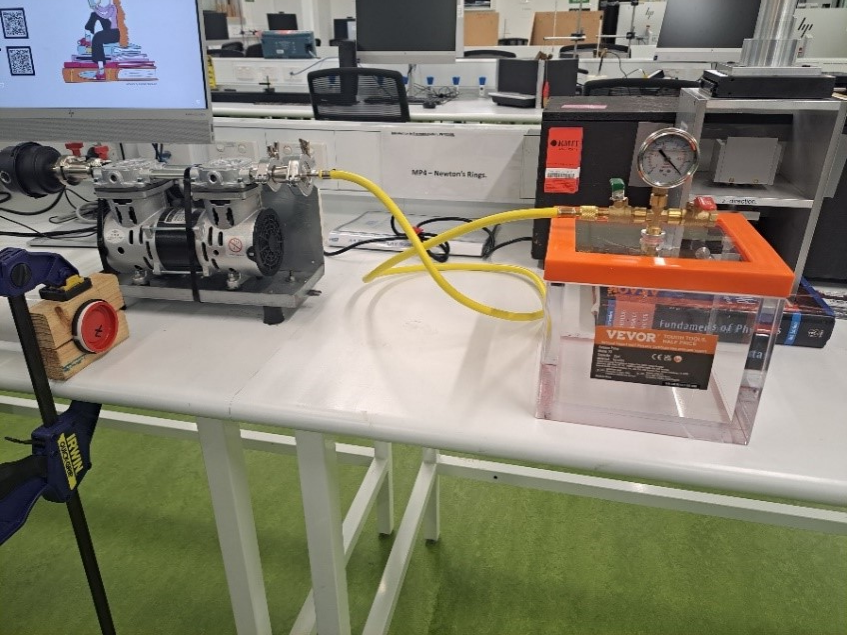
\includegraphics[width=0.85\textwidth]{./img/vacuum_chamber.png}
    \end{center}
    \caption{Experimental set up for vacuum chamber testing}\label{fig:vacuum_chamber}
\end{figure}

During the test, the vacuum pump gradually reduced the pressure, aiming for the target 78.36 kPa pressure. As the pressure approached this value, the system simulated apogee by maintaining the reduced pressure for a few seconds. To maintain this specific pressure for simulating apogee, the pressure leak was intentionally adjusted. 

This was achieved by fine-tuning the chamber’s pressure leak valve, allowing just enough air to enter the chamber to balance the amount of air being removed by the pump. By matching the air leak to the pump’s extraction rate, the pressure stabilised, holding at the desired level for a few seconds. The test ended with a slow depressurisation to simulate the descent back to ground pressure levels. 

Throughout the process, both data from the avionics system and the Blue Raven were collected for analysis. The key focus of the test was to validate the barometer’s ability to maintain accuracy throughout different pressure stages and verify the effectiveness of the calibration and apogee simulation process. Further experimental design details and risk assessments can be found under the Appendix~\ref{apdx:risk_assessment}. 

\subsubsection{Implications and Challenges}
The vacuum chamber experimental design faced several technical challenges, particularly with the Blue Raven flight computer. Firstly, there was difficulty placing the Blue Raven in a dedicated ground testing mode that would allow data collection for a set period of time. According to the user guide, there are no commands to set the hardware into a ‘launch’ mode, which led to serial communication via Real Term as a last resort to capture the data. While this method was effective for observing live sensor data, it presented a challenge as it required a wired connection through the chamber, which was not feasible within the testing period available. Figure~\ref{fig:realterm} displays the use of the RealTerm to connect serial to the Blue Raven via serial connection, outputting live senor data.

\begin{figure}[h]
    \begin{center}
        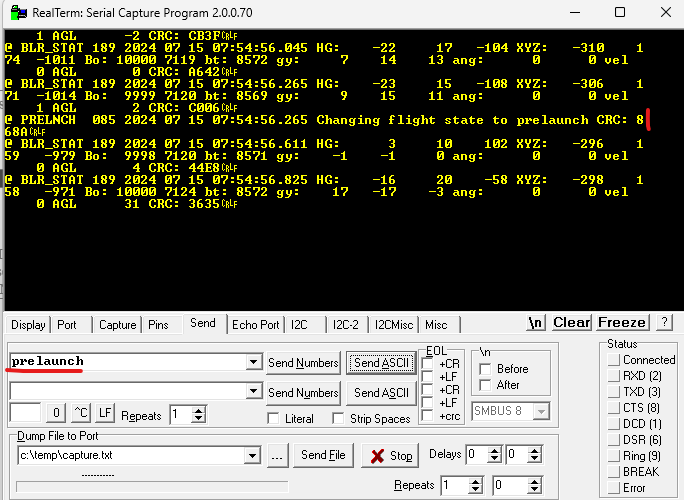
\includegraphics[width=0.75\textwidth]{./img/realterm.png}
    \end{center}
    \caption{RealTerm data output from Blue Raven}\label{fig:realterm}
\end{figure}

As a last resort, contact was made with Featherweight support who designed the Blue Raven Flight computers, who confirmed that no other method was available to place the Blue Raven into the required test mode. As a workaround, Featherweight’s Bluetooth app was used to monitor the pressure altitude as it output live readings of the current altitude. However, this solution had its limitations, as the app did not provide access to raw pressures data over time, but it served as a reasonable basis for comparison.  

Another challenge arose with the Pfeiffer vacuum gauge. The gauge had fitting inconsistencies with the chamber, which made it difficult to maintain a proper seal. Ultimately the original gauge built into the chamber was used to avoid further complications.

\subsubsection{Test \#1 Results}
The first barometric test using the vacuum chamber was conducted on 16th September. Throughout the test, various challenges and inconsistencies were encountered in the sensor readings. The barometer's pressure readings displayed sporadic noise, which introduced uncertainty to the data. For instance, the ground pressure was expected to be around 103 kPa, however the barometer consistently read approximately $\qty{90}{\kilo\pascal}$. This inconsistency persisted despite adjustments, such as changing the sensor’s orientation. 

When the barometer was faced upwards, the sensor showed a pressure increase towards the expected correct value. However, this behaviour introduced further uncertainty about the board's overall functionality. The shape of the data graph generated during the test closely matched expectations, but the actual pressure values remained inaccurate, deviating from the expected ~80 kPa target. 

\begin{figure}[h]
    \begin{center}
        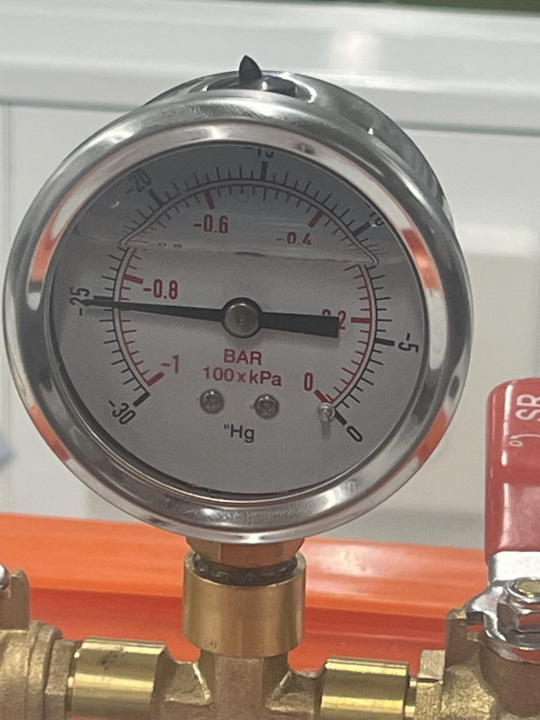
\includegraphics[width=0.45\textwidth]{./img/gauge.png}
    \end{center}
    \caption{Simulated apogee, where the pressure chamber levelled off and maintained pressure for a short period of time.}\label{fig:gauge}
\end{figure}

Referring to Appendix~\ref{apdx:vacuum_ground-raven}, which shows the ground pressure reading of the Blue Raven altimeter at $\qty{-29}{\feet}$, and Appendix~\ref{apdx:vacuum_peak-raven}, showing the recorded pressure altitude of $\qty{48,627}{\feet}$ during the simulated apogee, the results show a significant discrepancy in expected readings. Further analysis showed that while the system could track altitude changes, the pressure readings still presented challenges. 

Figure~\ref{fig:gauge} highlights the moment when the pressure chamber maintained a stable pressure to simulate apogee for a short moment, showing the effort to keep conditions stable during testing.

\subsubsection{Test \#2 Results}
The second set of vacuum chamber tests, conducted on 23rd of September, focused on evaluating both barometer accuracy and LoRa communication under simulated altitude conditions. As the pressure inside the vacuum chamber was gradually reduced to simulate an altitude of $\qty{49,000}{\feet}$ (as recorded by the BR system), the chamber maintained a pressure level consistent with this altitude reading. A3 Avionics system barometer recorded a pressure reading of $\qty{45.988}{\kilo\pascal}$ at altitude.  

However, an issue was observed with the barometer when the chamber was slowly being pressurised. Even after the chamber reached full pressurisation, the readings over LoRa remained stuck at around $\qty{67}{\kilo\pascal}$. This inaccurate reading persisted even after the chamber lid was opened, suggesting a problem with the barometer’s ability to detect pressure changes. 

LoRa communication, on the other hand, performed as expected throughout the test, transmitting data. Approximately three minutes after reaching altitude, the barometer in the A3 system suddenly adjusted to a reading of $\qty{71.5}{\kilo\pascal}$ over four samples, where it stabilised. However, this reading remained incorrect, as it should have been closer to the expected $\qty{103}{\kilo\pascal}$. Even after performing a power cycle, the barometer continued to display the same incorrect reading, highlighting a potential hardware malfunction. 

\begin{figure}[h]
    \begin{center}
        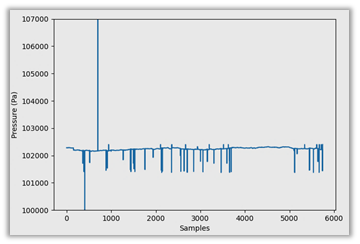
\includegraphics[width=0.65\textwidth]{./img/barometer_spikes.png}
    \end{center}
    \caption{Erroneous data in barometer readings}\label{fig:barometer_spikes}
\end{figure}

The accompanying pressure plot of a subsequent test, as shown in Figure~\ref{fig:barometer_spikes}, illustrates the inconsistencies and noise in the data, highlighting that some tests showed little to no changes in the pressure reading. These results indicate a need for further testing and hardware adjustments to ensure accurate pressure readings.

\subsubsection{Key Findings}
The findings from the vacuum chamber tests revealed a number of challenges and inconsistencies that impacted results that were collected. One of the most significant observations was the inconsistency in behaviour during each test, where the data varied unexpectedly and did not align with expected outcomes. This inconsistency highlighted the importance of understanding the hardware's limitations, especially when operating at the extremes of its performance capabilities, as outlined in its data sheet. 

A critical aspect of the testing procedure was the need to properly throttle the pressure within the vacuum chamber to simulate real-world altitude conditions. In future testing, the importance of using a more accurate pressure gauge became apparent, as the gauge used in these tests may have contributed to some of the inconsistent results. 

A primary issue identified during the testing was the potential for hardware failure. It remains unclear whether the barometer sensor was damaged during a previous drone crash during testing or if the unexpected pressure levels within the vacuum chamber contributed to its malfunction. Regardless, the malfunctioning barometer was replaced and tested outside of the chamber due to time constraints. These subsequent tests indicated that the replacement sensor was functioning as expected, producing accurate ground-level pressure readings. 

\subsection{RTOS Task Verification}
\subsection{Ground Communications Testing}
\subsection{State Estimation Verification}
\subsubsection{Drone Testing}
The objective of the drone testing is to validate the state transition logic for apogee detection in the avionics system of Aurora V. To simulate the ascent and apogee of a rocket flight, a drone test vehicle was configured with the SRAD flight computer, as shown in Figure~\ref{fig:drone} which was developed by the Avionics, Ground Communications, and Redundant Systems team~\cite{avionics}. The test involved monitoring state changes signalled by an LED on the flight computer, triggered when certain conditions were met during the drone's ascent. These conditions, which signify the transition from launch to coast and then apogee, were based on sensor fusion, utilising data from the onboard accelerometer, gyroscope, and barometer.

\begin{figure}[h]
    \begin{center}
        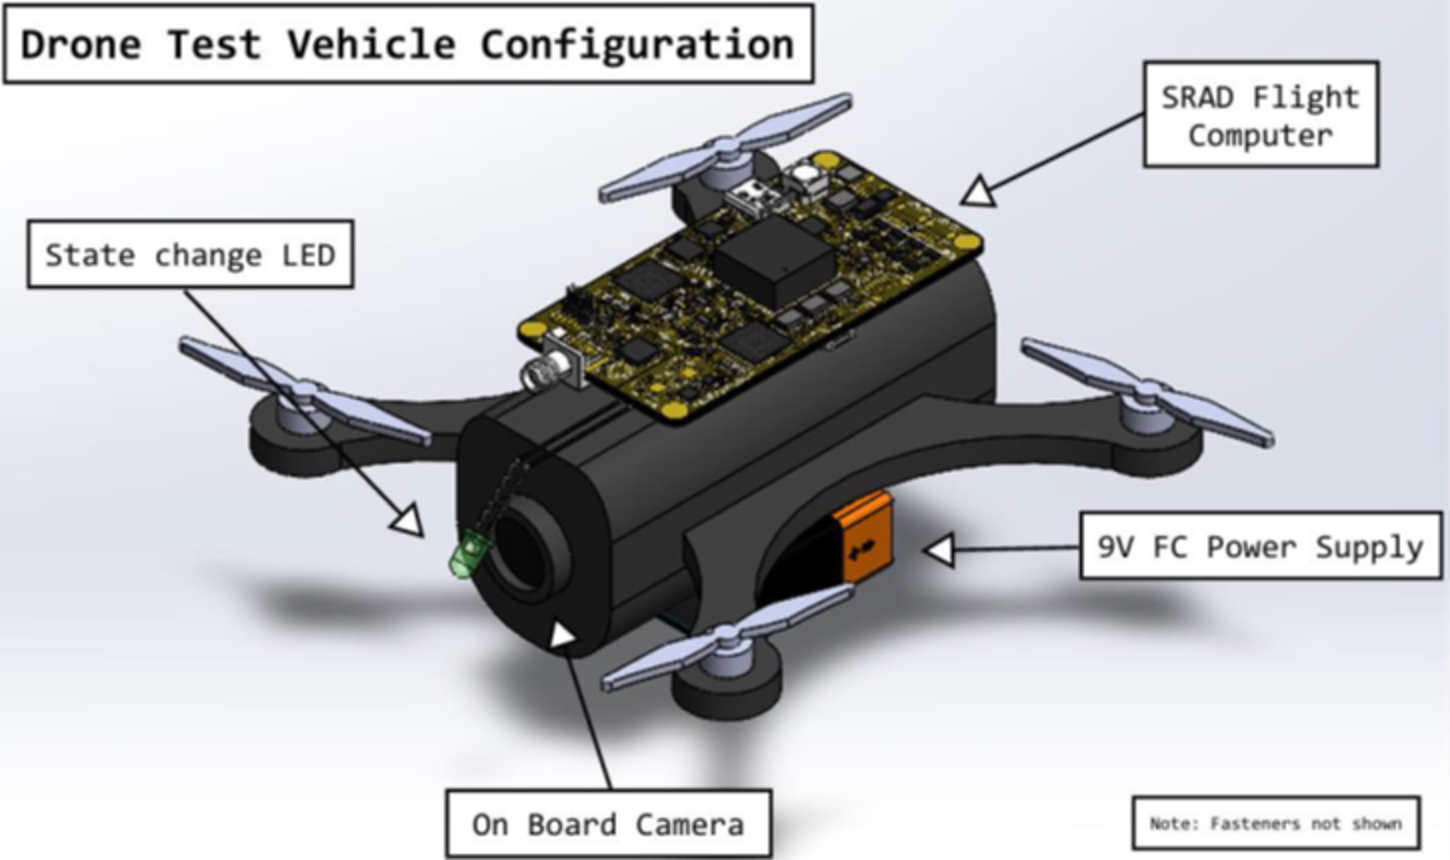
\includegraphics[width=0.85\textwidth]{./img/drone.png}
    \end{center}
    \caption{Drone test vehicle configuration}\label{fig:drone}
\end{figure}

The drone's flight mimicked key stages of a rocket's trajectory, starting with pre-launch, where the flight computer initialised and armed itself. This was followed by launch, which was triggered by the drone exceeding an acceleration threshold set to 2g for testing. During the coast phase, the flight computer detected a decrease in vertical velocity, signalling the drone's gradual deceleration towards apogee. 

For apogee detection, three key conditions had to be met: increasing barometric pressure, greater than 90-degree tilt from the initial launch axis, and sub-zero velocity. These were used to determine the exact moment of apogee. 

\begin{figure}[h]
    \begin{center}
        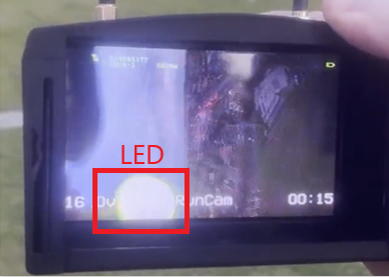
\includegraphics[width=0.75\textwidth]{./img/drone_led}
    \end{center}
    \caption{Live camera feed from the drone during flight}\label{fig:drone_led}
\end{figure}

A successful test was indicated by the LED toggling with each phase transition. Seven tests were conducted, successfully confirming the flight computer’s ability to accurately detect apogee under varying conditions including both with the drone tilting at apogee and without. Figure~\ref{fig:drone_led} shows the live camera feed from the drone, with the LED status visible. This verification process ensured that the avionics system was ready for integration into full-scale rocket launches. 

\subsubsection{Dummy Data Testing}

\section{Launch outcomes and Results}
\subsection{Aurora I}
The Aurora I launch was largely successful, especially considering the limitations in hardware availability. Data collection was performed post flight by reading the serial output from the onboard flash and converting the specified data frames into CSV format for further analysis. Although the barometric data was irretrievable due to a configuration error, we were able to use data from the Blue Raven as substitute for processing calculations when needed.  

\begin{figure}[h]
    \begin{center}
        \begin{minipage}{0.48\textwidth}
            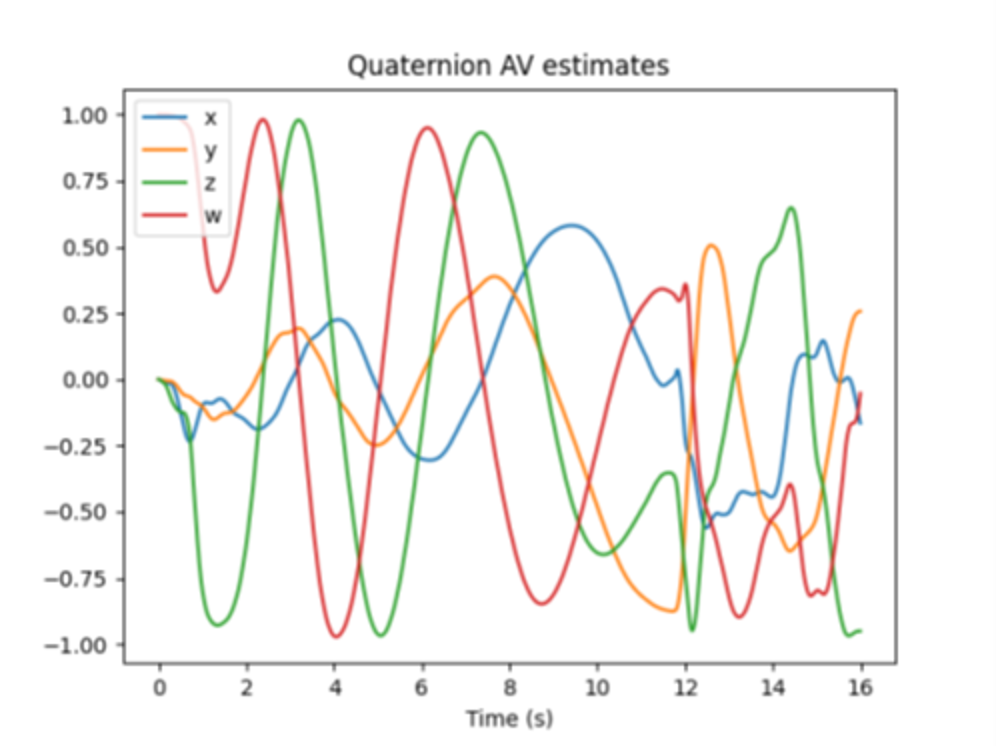
\includegraphics[width=\linewidth]{./img/quaternion_AV-A1.png}
        \end{minipage}\hspace{1em}%
        \begin{minipage}{0.48\textwidth}
            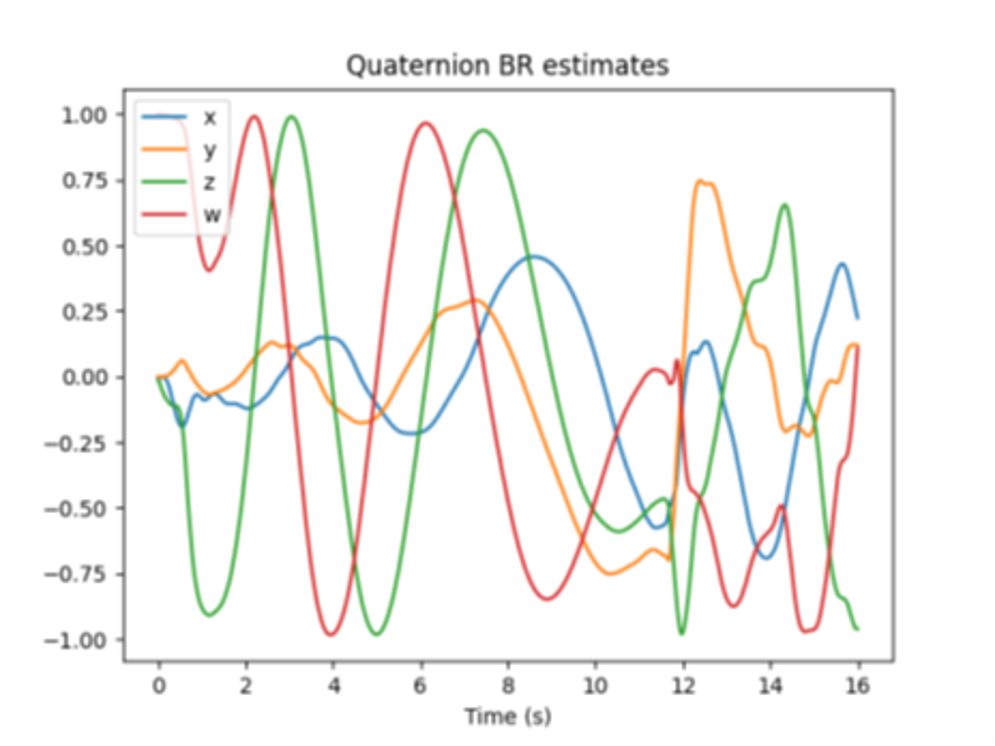
\includegraphics[width=\linewidth]{./img/quaternion_BR-A1.png}
        \end{minipage}
    \end{center}
    \caption{Comparison of quaternion estimates from A1 avionics and Blue Ravens}\label{fig:quaternion_A1}
\end{figure}

Upon analysis, the avionics system’s data output was generally consistent with the Blue Raven's data, as demonstrated in the high resolution accelerometer and gyroscope readings. Some noise artifacts were observed, likely a result of using backup components at short notice. However, these were mostly mitigated by the data processing techniques implemented, allowing us to retain meaningful insights.

In Figure~\ref{fig:quaternion_A1}, a comparison of quaternion estimates for the initial 14 seconds of flight illustrates a strong alignment between the avionics system’s attitude estimations and those of the Blue Raven, up until approximately t = 10.3 seconds when apogee was reached. While minor deviations in the x and y components were noted, these were within acceptable margins. Post apogee, the error margin widened, likely due to oscillations from recovery deployment and potential sensor impact from the deployment charges. 

\begin{figure}[h]
    \begin{center}
        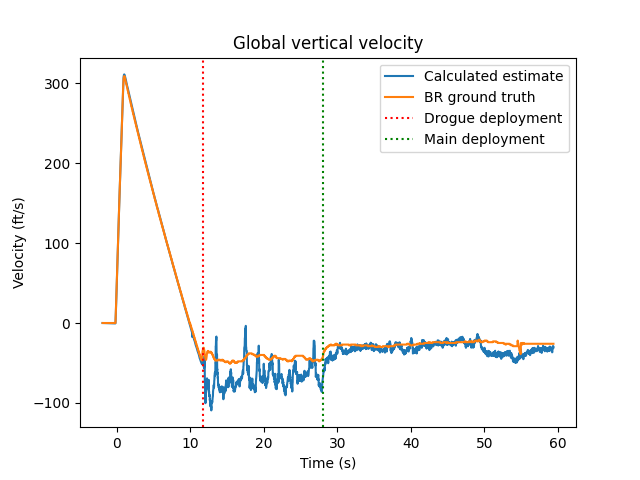
\includegraphics[width=0.75\textwidth]{./img/velocity_A1.png}
    \end{center}
    \caption{Calculated velocity from Kalman Filter compared to Blue Raven output}\label{fig:velocity_A1}
\end{figure}

Figure~\ref{fig:velocity_A1} illustrates velocity estimations produced by the Kalman Filter during ascent, drogue, and main chute deployment stages, which will be referred to as regions A, D, and M, respectively. Bayesian Optimisation was applied to recalibrate noise parameters Q and R within each region to improve the filter’s accuracy. 

The filter performed well in region A, which was critical for providing accurate data to other subsystems during ascent. However, it struggled in regions D and M, likely due to limitations in the current velocity model in addition to significant disturbances in the acceleration readings as a result of the rocket's erratic motion during descent under chute. Since accuracy in these regions primarily aids ground station visualisation post-deployment, addressing this limitation was at this stage a low priority.

\subsection{Aurora II}
The Aurora II launch continued with the same avionics system as Aurora I, with the primary modification being a firmware patch to enable logging of barometer data. This launch, initially which was originally cancelled, came together at the last minute in terms of structural preparation. Although data was successfully collected during the flight, no comprehensive analysis was performed, as the team’s focus had already shifted towards the development and preparation of Aurora III. 

The primary purpose of the Aurora II flight was to verify that the barometric sensor data would now be recorded, following the fixes made post-Aurora I. With sufficient data already gathered from the first launch, development of the Kalman Filter library for data processing had already begun. 

Consequently, the retrieved data from Aurora II was logged but remained unanalysed, serving instead as an additional validation point for the hardware modifications made. This allowed the team to concentrate resources on Aurora III, building on the foundational data and insights gained from Aurora I.

\subsection{Aurora III}
The Aurora III launch marked the first iteration of a RTOS within the avionics system. The RTOS allowed for both high and low-resolution data acquisition tasks, as well as data saving to flash storage. The RTOS was successfully integrated with these essential functionalities, but several challenges hindered the mission's success. 

One of the primary challenges encountered was related to the driver written for the on-board flash chip. The team attempted to diagnose the issue up to the day of the launch, but due to time constraints, a complete resolution could not be reached. 

To mitigate this issue, the team chose to utilise HAL (Hardware Abstraction Layer) libraries to interface with the device. HAL libraries are designed to provide a layer of abstraction between hardware and software, allowing developers to interact with hardware peripherals using a standardised approach without the need for low-level, hardware-specific code. Although these libraries can easily be integrated, they often include excessive bloat, with unnecessary code and dependencies that are not always required for specific systems like Aurora III. 

These libraries can slow down the performance and introduce unwanted complexities during debugging. For this reason, the team decided to develop custom drivers tailored specifically to our system requirements providing greater control over the code. Despite the driver appearing to work during initial tests using dummy data to save to flash, when the Aurora III was recovered post-launch, unfortunately no usable data had been recorded in the data frames. This posed a setback in data collection. 

In addition, other subsystems, such as state estimation, telemetry, and communication between the avionics and subsystems like the Aerobrakes, were not functional during the flight. This was despite successful communication tests the night before the launch. On the day of the launch, wire connection issues prevented the integration of these systems.  

A critical challenge throughout the process was the lack of time for thorough testing and validation. Last minute integrations and troubleshooting meant that the system could not be adequately tested in flight conditions prior to launch, leaving unresolved issues that ultimately affected the launch outcome.

\subsection{Aurora IV}
\begin{figure}[h]
    \begin{center}
        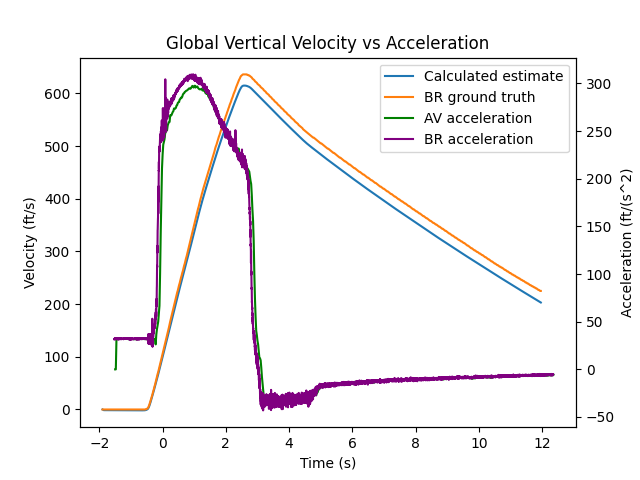
\includegraphics[width=0.75\textwidth]{./img/velocity_A4.png}
    \end{center}
    \caption{Kalman Filter state estimates for Auora IV launch}\label{fig:velocity_A4}
\end{figure}

\subsection{Aurora V}

\section{Challenges}
\subsection{Time Constraints and Delays}
Time constraints posed a significant challenge throughout the entirety of this capstone project. Although the launch schedule was relatively spaced out, the team underestimated the amount of time it would take for comprehensive testing and validation between each rocket launch. With each new launch date approaching there was a continual focus on implementing features, rather than refining and validating existing components. This lack of time for thorough testing increased the risk of software bugs and hardware issues going unnoticed until critical stages.  

In addition to time management issues, dealing with a wide range of stakeholders created unexpected delays. Coordination with other subsystems, including the Aerobrakes and Payload teams, often required additional time to ensure integration went smoothly. Moreover, receiving support and approval from RMIT technical staff, particularly for laboratory equipment such as the vacuum chamber and shake tables, involved lengthy administrative processes. These approvals and technical consultations often took longer than anticipated, adding more pressure to the project timeline. 

Furthermore, delays in receiving avionics hardware components especially for the Aurora III board further put pressure on the team, as the hardware was required to integrate and assess firmware. The limited number of flight boards available meant that only one or two developers could work on the avionics system at a time, restricting the pace of progress. In particular, the team’s reliance on the Avionics, Ground Communications, and Redundant Systems team for board access often resulted in delays, leaving less time for development, integration, and testing.  

\subsection{Hardware Availability}
\subsection{Collaboration}
\subsection{Erroneous Data and Logic Errors}

\section{Recommendations and Future Work}
\subsection{Suggested Improvements}
There are several major areas that remain for improvement to ensure ideal operation of the avionics system from a data analysis and verification perspective. One key design goal that was unfortunately not realised is the firmware implementation for full redundancy on the latest iteration of the Aurora V avionics, with internal communication across dual redundant microcontrollers for mid-flight fail-safes. The implementation of this redundancy has not yet been fully realised and should be a top priority moving forward.  

Looking ahead to the 2025 competition team, attention should focus on refining the avionics sensor systems and telemetry for more accurate data transmission and real-time flight monitoring. In the Aurora V launch, these systems did not function as expected, resulting in no ground communications. Further validation of LoRa communication in an integrated setting is recommended.  

From a sensor testing point of view, it is suggested future team utilise a Clinostat, a ground-based testing rig designed to simulate key flight conditions, such as pitch, yaw, and roll. This setup will allow future teams to conduct comprehensive tests of avionics components and gyroscopes under controlled conditions, reducing the need for full-scale flight tests before hardware integration. For more laboratory-based test such as using vacuum chambers and shake tables, future teams are advised to develop experimental designs well in advance of launch and create a plan to ensure that testing is conducted as firmware is developed. Although tests were conducted in this capstone, most validation was conducted after launches which was not ideal.  

Additionally, maintaining code documentation will be a component of the ongoing work. The current code has been structured in a modular fashion, making it easier for future students and teams to build upon the existing foundation. Continuing this practice will enable smoother transitions between teams and ensure that each subsequent group can quickly pick up where the previous one left off, improving development continuity.

\subsection{Further Development}

\section{Conclusions and Learning Outcomes}
To close out, this capstone project marked a significant achievement in advancing the Aurora V rocket, culminating in the development of a comprehensive, student-designed avionics system. Collaborating closely with the rest of the Aurora sub teams, we were able to design, test, and successfully launch five high-powered rockets, integrating all key avionics deliverables from data acquisition to state estimation. The avionics system now features a custom Real Time Operating System firmware that efficiently manages real time data capture from accelerometer, gyroscope, and barometer sensors. Additionally, we developed a custom library for data processing and state estimation, validated through testing, including vacuum chamber trials for barometer accuracy and drone tests to verify apogee detection. 

Although LoRa communication didn’t operate as expected on launch day, real-time data transmission between the rocket and ground has been implemented from a firmware perspective and should be further tested for future launches. A key milestone of this project was the successful recovery of flight data, an essential component for post launch analysis. Ultimately this project serves as a solid foundation for future teams, positioning future teams who enter the AURC to achieve even greater milestones in rocket avionics and telemetry. The team's dedication and collective effort have set a new standard for student driven rocketry projects at RMIT. 

\section{Acknowledgements}
As members of the 2024 AURC Aurora V Avionics team we wish to acknowledge our incredible capstone supervisor, Dr. Glenn Matthews, without whose invaluable support and guidance we likely would not have come as far in our endeavours. 

Throughout the year Glenn has gone above and beyond in his involvement with the team, attending many of our launches and showing a level of support for his students and for the project greater than we have seen from any other academic. With his assistance we managed to overcome many obstacles and have learned much more than we could have expected.

\begin{figure}[h]
    \begin{center}
        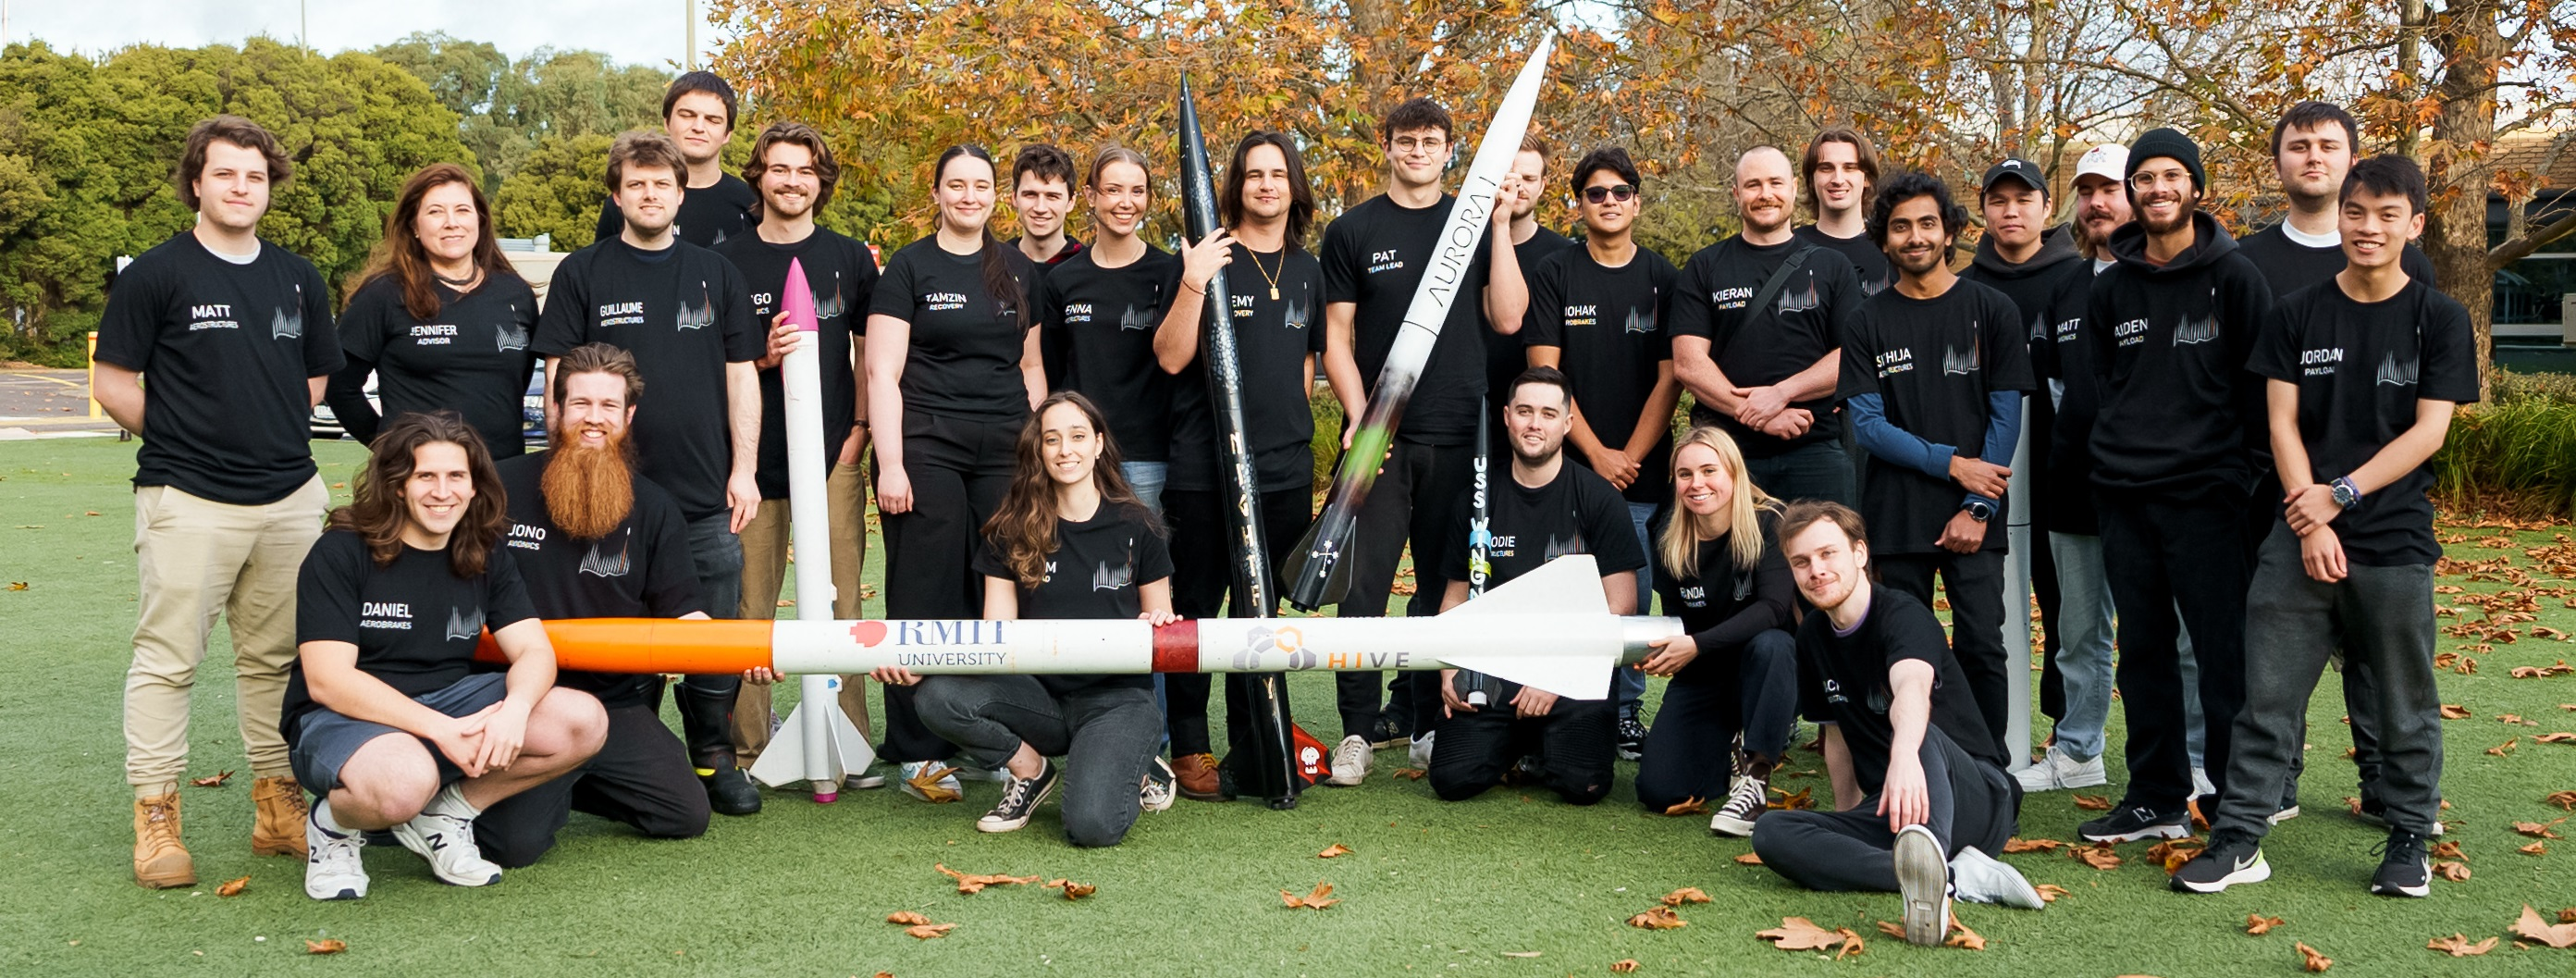
\includegraphics[width=\textwidth]{./img/aurora_team.jpg}
    \end{center}
    \caption{AURC Aurora V team 2024}\label{fig:aurora_team}
\end{figure}

We would also like to extend our gratitude to the greater Aurora team, for the amazing opportunity and experience this past year. We have come a long way since the beginning of this project, and through the ups and downs have managed to build and launch five rockets from the ground up. 

\hfill{}\textbf{Thank You}\hfill{}

\vfill{}\hfill{}P.S. Our rockets went brrr...
